\subsubsection{Administrationsbereich}
\label{sec:UmsetzungAdministrationsbereich}

Der entwickelte Prototyp stellt eine erste lauffähige Version der
Benutzeransicht dar. Der nächste Entwicklungsschritt ist die Implementierung
des Administrationsbereichs und die Bereitstellung von APIs. Aufbauend auf
Informationen im Administrationsbereich wird der Prototyp anschließend um
dynamische Funktionalität erweitert. Hierbei werden die angezeigten
Panoramafotos und die benachbarten Panoramafotos über eine API angefragt,
welche die Informationen aus der Datenbank lädt. Der Implementierungsprozess des
Administrationsbereiches wird dabei sukzessiv anhand der vorgestellten
Anwendungsfällen im \verweis{Adminstratoranwendungen} auf Seite
\pageref{sec:Adminstratoranwendungen} realisiert. Prioresiert werden dabei die
Anwendungsfälle, die die Verwaltung der Panoramas, Infotexte und die
Übersichtskarte betreffen (AFA05 bis AFA17).

Bevor mit der Implementierung begonnen werden kann wird ein einheitliches
Design festgelegt, welches den späteren Administratoren das Verständnis der
Administrationsfunktionen erleichtern soll. Zu diesem einheitlichen
Designkonzept zählt zum Beispiel das Farbschema der Buttons. So wurde
beispielsweise festgelegt, dass ein roter Button immer das Löschen und ein
grüner Button immer das Speichern eines Datensatzes signalisiert. Darüber hinaus
wurde entschieden, die Gestaltung von Buttons, Informationsfenster und
ähnlichem mit dem CSS\footnotemark\ Framework Bootstrap\footnotemark\ zu realisieren.
Dadurch ist gewährleistet, dass alle Steuerelemente in allen Browsern
gleich aussehen. So kann der Administrator Steuerelemente anhand der Gestaltung
wiedererkennen und über die Gestaltung auf deren Funktion schließen. Hierdurch
wird die Usability der Software erhöht.

\footnotetext{CSS steht für Cascading Style Sheets und beschreibt eine
Skriptsprache, die dazu dient HTML-Elemente in Form und Farbe zu verändern.}

\footnotetext{Bootstrap ist ein Open Source Projekt, in dem einheitlich das
Design von verschiedenen HTML-Elemente definiert ist. Bootstrap ist ein Projekt
des Internetkonzerns Twitter und ist besonders dafür geeignet, ein einheitliches
Look and Feel einer Webseite in allen Browsern zu erzeugen.}

Aufbauend auf den Administrator-Anwendungsfällen und dem Designkonzept werden
Arbeitspakete erstellt, welche sich auf die Implementierung der
Informationstext- und Fotoverwaltung beziehen. Zur Verdeutlichung der
eingesetzten Technologien und des Entwicklunsablaufs wird im Folgenden eine
stark vereinfachte Fotoverwaltungsseite implementiert. Hierbei soll eine Seite
erstellt werden, die alle Fotos der Datenbank mit Namen und Beschreibung
anzeigt. Zustätzlich soll es dem Administrator möglich sein, auf den Namen eines
Fotos zu klicken, um weitere Informationen zu dem Foto einzusehen.

Zur Implementierung dieses Szenarios wird zunächst ein HTML-Dokument
angefertigt, welches das Grundgerüst der Fotoverwaltung darstellt. In diesem
Grundgerüst können bestimmte Elemente, wie zum Beispiel die
Navigationsbar\footnote{Vergleiche \abbildung{MockupBackend}} am oberen Rand der
Seite oder der Titel der Seite, statisch erstellt werden. Zur Vereinfachung soll
aber nur der Titel der Seite und eine Überschrift festgelegt werden. Das
\listing{HTML_Anwendungsbeispiel} zeigt das beschriebene HTML-Dokument.

\lstinputlisting[language=HTML,caption={statisches
HTML},label={lst:HTML_Anwendungsbeispiel}]{Listings/HTML_Anwendungsbeispiel.html}

Im Anschluss muss die Seite um dynamisch generierten Inhalt erweitert werden.
Dynamischer Inhalt ist im gegeben Anwendungsfall das Anzeigen aller Fotos, die
bereits in der Datenbank gespeichert sind. Um dieses Verhalten zu realisieren
muss eine Anfrage an die Datenbank gestellt und für jeden Eintrag in der
Datenbank HTML-Quellcode geschrieben werden. Das \listing{HTML mit PHP} zeigt
diese Implementierung in PHP.

\lstinputlisting[language=HTML,caption={Dynamisches schreiben von HTML mit
PHP},label={lst:HTML mit PHP}]{Listings/HTML_mit_PHP.php}

Dargestellt ist die Anfrage an die Datenbank, die durch die PHP-Funktion
"`mysql\_query"' (Zeile 5) realisiert wird, das Durchlaufen jedes
Datenbanksatzes in einer Schleife (Zeile 6ff.) und das Schreiben von HTML mit
dem PHP "`echo"'-Befehl.

Zum Abschluss wird das Klicken auf den Fotonamen implementiert. Diese
Benutzerinteraktion kann am besten auf dem Clientsystem des Benutzers
mit Javascript verarbeitet werden, da keine weiteren Informationen vom Server
benötigt werden. Auf diese Weise werden zusätzliche Serveranfragen vermieden.
Javascript-Routinen werden meistens als Funktionen formuliert, die aufgerufen
werden, wenn ein bestimmtes Ereignis eintritt. In \listing{HTML mit PHP} ist
ein solcher Funktionsaufruf in Zeile 9 dargestellt. Die Funktion
"`toggleDescription"' wird aufgerufen, sobald auf das <p>-Tag geklickt wird. Als
Parameter wird dieser Funktion das eigene HTML-Element, also das <p>-Tag,
übergeben. Die Javascript-Funktion ist in \listing{JavascriptSnippet}
dargestellt.

\lstinputlisting[language=JavaScript,caption={Auf Benutzerinteraktion reagieren
mit Javascript},label={lst:JavascriptSnippet}]{Listings/Javascript_Snippet.js}

Alle dargestellten Listings könnten in einem Dokument stehen, welches vom dem
Administrator über seinen Internetbrowser angefragt wird. Wie bereits erwähnt
ist diese Darstellung der Implementierung stark vereinfacht. Die Quelldateien,
die die Fotoverwaltung im vorliegenden Projekt implementieren, sind zu
umfangreich, um an dieser Stelle präsentiert werden zu können. Die
implementierte Fotoverwaltung ist in \abbildung{Fotoverwaltung} dargestellt.

\begin{figure}[htb]
\centering
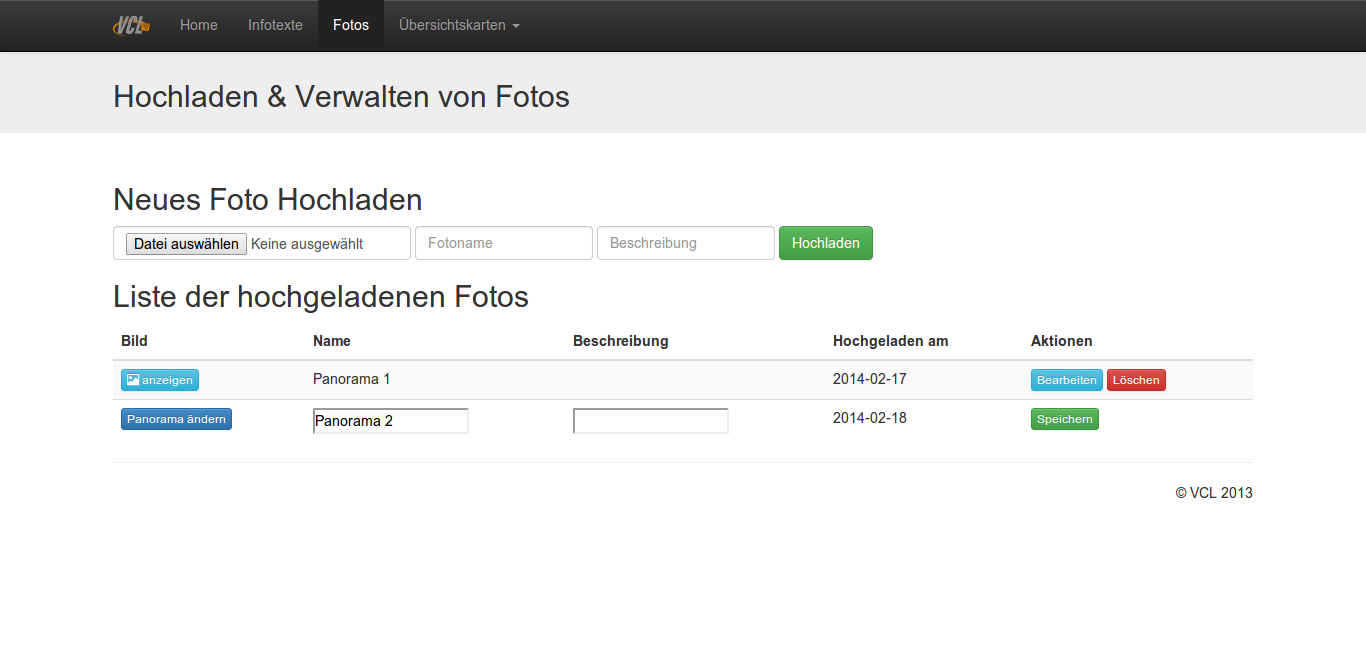
\includegraphics[width=1.0\textwidth]{Fotoverwaltung.png}
\caption[Fotoverwaltung]{Bildschirmfoto der implementierten Fotoverwaltung}
\label{fig:Fotoverwaltung}
\end{figure}

In dem zuvor beschriebenen Entwicklungszyklus wurde auch die Verwaltung der
Infotexte und die Übersichtskarte implementiert. Bildschirmfotos dieser Bereiche
sind im Anhang \ref{sec:BildschirmfotoInfotextverwaltung}
(\nameref{sec:BildschirmfotoInfotextverwaltung}) auf Seite
\pageref{sec:BildschirmfotoInfotextverwaltung} und im Anhang
\ref{sec:BildschirmfotoUebersichtskarte}
(\nameref{sec:BildschirmfotoUebersichtskarte}) auf Seite
\pageref{sec:BildschirmfotoUebersichtskarte} dargestellt. Mit dem Abschluss der
Implementierung dieser Bereiche ist der Administrationsbereich fertiggestellt.